\documentclass[prodmode,acmtecs]{acmsmall} % Aptara syntax

% Package to generate and customize Algorithm as per ACM style
\usepackage[ruled]{algorithm2e}
\renewcommand{\algorithmcfname}{ALGORITHM}
\SetAlFnt{\small}
\SetAlCapFnt{\small}
\SetAlCapNameFnt{\small}
\SetAlCapHSkip{0pt}
\IncMargin{-\parindent}

% Metadata Information
\acmVolume{000}
\acmNumber{000}
\acmArticle{000}
\acmYear{2015}
\acmMonth{12}

% Copyright
%\setcopyright{acmcopyright}
%\setcopyright{acmlicensed}
\setcopyright{rightsretained}
%\setcopyright{usgov}
%\setcopyright{usgovmixed}
%\setcopyright{cagov}
%\setcopyright{cagovmixed}

% DOI
\doi{0000001.0000001}

%ISSN
\issn{1234-56789}

% Document starts
\begin{document}

\newcommand{\titleNameLong}{General-Purpose Computing on GPUs and Efficient
Parallel Processing of Heterogeneous Applications}

\newcommand{\titleNameShort}{GPGPU and Efficient Parallel Processing of
Heterogeneous Applications}

% Page heads
\markboth{C. Smith}{\titleNameShort{}}

% Title portion
\title{\titleNameLong{}}
\author{Connor Smith
\affil{Brigham Young University}}

\begin{abstract}
This article is a survey of the current state of general-purpose computing on
GPUs (GPGPUs) and the use of heterogeneous applications on them. The underlying
architecture of GPUs is well-suited to problems with a high level of data
parallelism and has traditionally been used for rendering computer graphics.
Performing general-purpose computing on GPUs is a relatively recent development,
having only become practical and popular in the past decade or so. A brief
overview of a typical GPU architecture is presented, and the challenges of
applying this architecture to heterogeneous problems are discussed. Several
different current areas of research are explored, including dynamic warp
scheduling and hardware tuning, reducing memory contention, and software
solutions to the challenges of GPGPU. While the challenges presented are
difficult to overcome, general-purpose computing on GPUs continues to make
progress in the areas of performance, energy, and power.
\end{abstract}

\keywords{General purpose graphics processing unit, heterogeneous systems, warp
size, dynamic warp, GPU compression, hardware worklists, locality aware mapping}

\acmformat{\titleNameLong{}.}

\begin{bottomstuff}
This work is supported by the National Imaginary Science Foundation, under grant
CNS-0123456.

Author's address: C. Smith, Electrical and Computer Engineering Department,
Brigham Young University.
\end{bottomstuff}

\maketitle


\section{Introduction}
The purpose of this survey is to provide an introduction to general-purpose
computing on graphics processing units (GPGPU), the challenges inherent to this
field, and some active areas of research within the field to alleviate some of
these problems. To the best of the author's knowledge, this is the first survey
in this semester's course to discuss GPGPU.

The term GPU was popularized around the turn of the 21st century by NVIDIA as
consumer-level devices began to need dedicated accelerators to render 3D
graphics. Today, most all computers contain GPUs, from supercomputers to
laptops, desktops to smartphones, although some of these do not use dedicated
graphics cards. The area of GPGPU started to take off roughly a decade ago when
it began to be practical to solve traditional problems with the massively
parallel nature of GPUs. Using hundreds or even thousands of ``cores" to perform
computations in parallel is tempting (even if the cores are not really cores at
all), but brings with it a new set of challenges.

In a way, the problems of GPGPU are an extension of those sometimes seen in a
traditional desktop multiprocessing system. Even when under a heavy compute
load, it is not easy to keep all of the cores doing useful work in any given
cycle. Between limitations in structural units, dependences between
instructions, and latencies of memory accesses, the processor cannot help but
stall sometimes. This problem is exacerbated by orders of magnitude when solving
heterogeneous problems on a GPU. GPUs were originally designed to operate on
graphics processing, problems that are well-structured and have simple, inherent
data parallelism. Problems that do not contain parallelism that is easily mapped
to the architecture of a GPU fail to keep all of the cores in a GPU busy or
strain the memory bandwidth past the GPU's ability to hide latency.

The remainder of this survey is organized as follows. Section
\ref{sec:architecture} provides a brief architectural overview of GPUs. Section
\ref{sec:challenges} elaborates on the challenges specific to GPGPU
applications. Section \ref{sec:dynamic} discusses spawning granular helpers to
increase performance. Section \ref{sec:scheduling} deals with more efficient
scheduling within and among streaming multiprocessors, as well as tuning
hardware to match the current load of the GPU. Section \ref{sec:memory} talks
specifically about reducing memory contention. Section \ref{sec:software} is a
discussion of a few software and compiler solutions to the challenges of GPGPU.
Section
\ref{sec:conclusions} concludes the survey.

\section{Architectural Overview} \label{sec:architecture}
\subsection{Streaming Multiprocessors}
Modern unified GPUs consist of multiple streaming multiprocessors (SMs). Figure
\ref{fig:baseline} shows a baseline GPU configuration
\cite{DynamicThreadBlockLaunch}. While there are many GPU architectures
available today, the following description is based off of NVIDIA's Maxwell
architecture, which was released in 2014. These SMs are similar to SIMD
processors and typically contain the following components:
\begin{description}
  \setlength\itemsep{0.5em}
  \item[A large register file] The register file is shared across all threads
  and typically contains thousands of registers, many more than are usually
  found in a CPU. NVIDIA's Maxwell architecture has 64K 32-bit registers in each
  SM.
  \item[Multiple caches] Maxwell includes a unified L1/texture cache, which used
  as a coalescing buffer for memory accesses. The buffer gathers requested data
  and sends the entire group to a warp. There are also additional caches TODO.
  \item[Shared memory] There are 96KB available per SM in Maxwell. However,
  thread blocks are limited to 48KB each. Shared memory for a thread-block is
  only accessible by threads within the same thread-block.
  \item[Multiple warp schedulers] Warp schedulers dispatch and allocate
  resources. Maxwell contains four schedulers per SM, and functional units are
  assigned to a particular scheduler. Using a power-of-two number of CUDA cores
  per SM allows for simple partitioning among schedulers. One ready warp is
  scheduled per cycle, which allows the GPU to hide the latency of stalled
  warps.
\end{description}

\subsection{Kernels, Thread-blocks, and Warps}
A kernel is a potentially massive number of threads executing same piece of
code. From the application programmer's point of view, a function is called on
the device with a certain number of blocks and a certain number of threads
within each block. The CPU launches GPU kernels by dispatching launch commands.
Kernel parameters are passed from the CPU to the GPU at launch time and are
stored in the GPU's global memory. Kernels from different streams are
independent and can be run concurrently, but kernels within a stream are
sequential.

Grids are what actually run on the GPU, and they are composed of multiple
``thread-blocks'', also called a cooperative thread array (CTA) outside of
NVIDIA's nomenclature. Maxwell supports up to 64K blocks within a grid.
Thread-blocks contain potentially many threads, on the order of 1024 for modern
architectures. Each thread within a thread-block has the same life-cycle as all
the others, meaning that they are dispatched to and swapped from a SM at the
same time.

Individual threads exist within a thread-block. These threads are grouped into
``warps'', usually around 32 at a time. The warp is the fundamental unit of
execution on GPUs. Threads within a warp are mapped to a vector functional unit
such that all threads execute the same instruction on different data, just a
like a SIMD unit. With this in mind, it would be more accurate to call
``threads'' a sequence of SIMD lane instructions, but this survey will continue
to refer to them as threads to maintain consistency with the literature. The
term ``warp'' is the term used by NVIDIA, while AMD and OpenCL use
``wavefront''. Maxwell supports up to 64 warps resident per SM. Note that this
does not mean that all 64 warps are executing at the same time, but that the
architecture can support that many warp contexts concurrently. The SM maintains
a warp pool to store the context of all running threads. Warps are scheduled by
the warp schedulers from this pool.

\begin{figure}
  \centering
  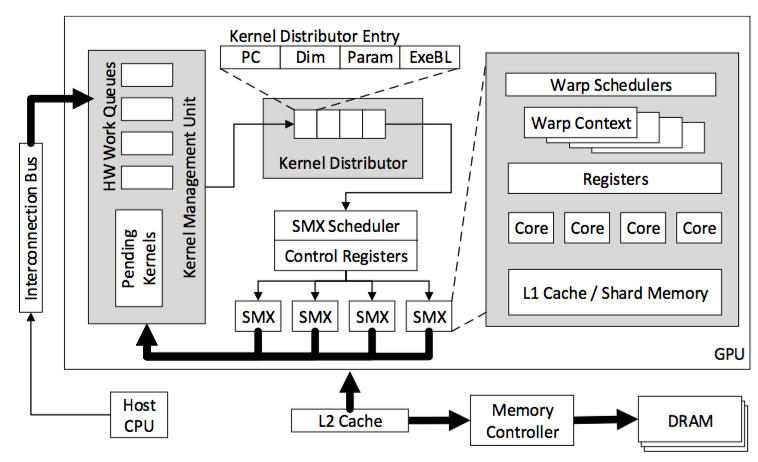
\includegraphics[]{BaselineGPU.png} \caption{Test caption} \label{fig:baseline}
\end{figure}

\section{Challenges of GPGPU} \label{sec:challenges}
\subsection{Heterogeneous Applications}
There are two main challenges of GPGPU. The first is maintaining high
performance on heterogeneous applications. As mentioned previously, this problem
is difficult simply due to the complicated structure of these applications. When
a warp stalls for one reason or another, the warp scheduler selects a new warp
to take its place the next cycle. This is an attempt to hide the latency of warp
stalls. However, GPU schedulers are limited in their ability to hide latencies
for heterogeneous applications. This is caused by imbalanced workloads among
warps, divergent branches, irregular memory accesses, and shared cache
contention \cite{CoordinatedWarpScheduling}. Designs in the following section
discusses these issues and present possible solutions.

\subsection{Memory Limitations}
The second challenge for GPGPU is mitigating memory bandwidth bottlenecks. A
majority of general-purpose applications run on GPUs are memory bound
\cite{AssistWarps}, which means that performance is bottlenecked by off-chip
memory bandwidth. This bottleneck is commonly due to contention among warps
within the GPU, and may also be a result of contention with memory use by the
CPU in heterogeneous system architectures
\cite{ManagingConcurrencyInHeterogeneous}. A number of schemes have been
suggested to reduce pressure on off-chip memory and will be visited in the next
section.

\section{Dynamically-Launched Helpers} \label{sec:dynamic}
\subsection{Assist warps}
As we have seen, GPUs are capable of supporting thousands of threads, but
bottlenecks in heterogeneous applications limit performance. Core-Assisted
Bottleneck Acceleration \cite{AssistWarps} is a scheme that uses ``assist
warps.'' These special warps are generated by dedicated hardware and are used as
helper threads to increase performance and efficiency. Assist warps share the
same context as the parent warp and uses some of the available registers, since
investigation shows that 24\% of the register file is unallocated on average.

One primary use for assist warps is memory compression. Instead of using
dedicated hardware for compressing and decompressing data from memory, this
approach uses existing hardware that is not being utilized. Another advantage of
not using dedicated hardware is the ability to change compression algorithms
flexibly, since different applications have varying access patterns that are
suited for different compression algorithms. Assist warps can also be used for
memoization, in which frequently-computed values from main memory are cached and
used as lookup tables, reducing the number of loads and stores required. One
final use suggested by the authors is using an idle memory pipeline to prefetch
values during computation to reduce the memory pressure.

CABA contains a mix of hardware and software. While software-only or
hardware-only options are possible, the former induces high overhead and
complicates communication between primary and helper warps, and the latter makes
having a flexible interface more difficult. The combination suggested by the
authors dynamically inserts instructions into the execution stream in the form
of assist warps. This requires stores of commonly used assist warps, a
controller to trigger and manage assist warp execution, and an assist warp
buffer inside the instruction buffer that holds triggered warps until they are
scheduled. Helper threads share context with the parent warp, and register
values in helper threads are not preserved between invocations, reducing the
overhead of this technique and does not require any additional resources.

The authors report a reduction in memory bandwidth of 2.1x, resulting in an
increase in performance of 41.7\%. This is only 2.8\% less than the idea case in
which there would be no overhead of assist warps. These helper threads also
reduced the overall system energy by 22.2\%, which is 4.0\% over the ideal
effect. Power consumption is also increased by 2.9\%, but this is a small price
to pay for the performance increases.

\subsection{Dynamic Thread Block Launch}
The authors of Dynamic Thread Block Launch (DTBL) suggest a somewhat similar
approach, this time launching thread blocks dynamically instead of assist warps
\cite{DynamicThreadBlockLaunch}. The motivation behind this technique is that
while emerging general-purpose applications do not have a simple, regular
structure that is easy to exploit at the highest level, they still do contain
``pockets'' of parallelism at smaller levels. The authors explain that these
pockets can be exploited with existing architecture using device-side nested
kernel launching, but at a high cost. For example, CUDA supports parent kernels
launching child kernels through device-side API calls. These child kernels can
start at any time after being launched by their parent. This method does exploit
pockets of parallelism, but this CUDA method results in an average of 36.1\%
decrease in performance, and also consumes significant amounts of memory by
storing pending child kernels.

The problems with existing implementations reduce down to four characteristics:
\begin{description}
  \setlength\itemsep{0.5em}
  \item [High kernel density] Kernel launches are expensive, and typical
  applications currently require many kernels. For example, a typical
  breadth-first search requires about 3,000 device kernel launches, resulting in
  a high overhead and memory footprint.
  \item [Low compute intensity] While many kernels are launched using these
  methods, they are usually fine-grained and do not contain high amounts of
  parallelism. The average number of threads in these kernels is around 40, which
  is close to the warp size and could be better served by a more fine-grained
  approach.
  \item [Workload similarity] The operations performed by each dynamically
  launched kernel are usually similar, but contain different levels of parallelism
  due to differing configurations or data.
  \item [Low concurrency/scheduling efficiency] Due to the low compute intensity
  of the device kernels, multiple kernels should be able to execute in parallel.
  However, GPU architectures place limits on the number of different kernels that
  can execute concurrently, and since each kernel has a relatively small number of
  warps within it, the SMs are underutilized and struggle to hide memory
  latencies.
\end{description}

DTBL is a more fine-grained approach. Instead of launching entire kernels,
individual thread blocks are created and added to the list of existing thread
blocks within a kernel. These thread blocks are coalesced into an aggregated
kernel and executed together. The existing GPU microarchitecture is extended to
support these additional thread blocks by adding data structures to keep track
of dynamically formed groups of thread blocks and associating them with kernels.
Fortunately, this organization is transparent to much of the rest of the
architecture, including the warp schedulers and control divergence mechanism.

The extra data structures of this technique only contribute an area overhead of
0.5\%. Additionally, the authors report a 1.21x performance increase over
original GPU implementations and 1.40x over implementations using existing
device-kernel launches.

\section{Dynamic Scheduling} \label{sec:scheduling}
\subsection{Critical Warps}
GPUs manage to hide latency by swapping out stalled warps, but current
performance is not good enough. This latency hiding is limited by the following
characteristics of heterogeneous applications: imbalanced workloads in parallel
warps, diverging branch behavior, irregular memory access patterns, and shared
cache contention \cite{CoordinatedWarpScheduling}. These imbalances and
irregularities result in differences in execution time of parallel warps. The
slowest warp in a group is called the ``critical'' warp. Since warps are blocked
for synchronization purposes until all of them are finished, this needlessly
extends the life of all the other warps and limits the performance of the
application as a whole. The authors of Criticality-aware warp acceleration
(CAWA) demonstrate that the average difference in execution time between the
fastest and slowest warp is 45\% and can reach as high as 70\%.

CAWA seeks to reduce the disparity among execution time in parallel warps using
three components:
\begin{description}
  \setlength\itemsep{0.5em}
  \item[Dynamic warp criticality prediction] This predictor attempts to identify
  the critical warp that is used in the next two components. This is
  accomplished by using a per-warp criticality counter, which is based on the
  degree of instruction count disparity, a measure of how much diverging
  branches differ, as well as the number of stall cycles between two consecutive
  instructions. These two values are combined into a single criticality counter.
  \item[A greedy criticality-aware warp scheduler] This scheduler is built on
  top of the two existing warp scheduling policies, and gives more time to
  critical warps (based on the criticality counter described above). Ties are
  broken by the age of the warp, giving priority to older warps.
  \item[Criticality-aware cache prioritization] This scheme prioritizes cache
  accesses. It reserves a fixed number of L1 data cache ways for critical warps.
  The best number of ways to reserve was determined by experimental analysis and
  found to be 8 out of 16. The cache prioritization also uses a signature-based
  hit predictor to predict whether a given cache line belongs to the critical
  warp.
\end{description}

Using an oracle to identify the critical warp could yield a 21\% performance
improvement on average. The use of CAWA resulted in an average improvement of
9.2\% across all applications. Applications that are more sensitive to
scheduling policies and cache accesses saw a 23\% improvement in performance.
The accuracy of the critical warp identifier was also measured. It successfully
identified the critical warp as a slow warp 73\% of the time, where slow warp
here means it is in the slower half.

\subsection{Variable Warp Size}
While some of the past sections have discussed added new execution objects to
perform work, this technique pertains to splitting and re-merging existing warps
\cite{VariableWarpSize}. There are two types of divergence in GPU execution:
control flow divergence and memory divergence. The former deals with complex
control flow in large warps resulting in performance loss, while the latter is
related to how well memory requests are coalesced into single warps. When warps
are too small, horizontal locality of memory accesses is lost; this effect is
termed ``memory convergence slip.''

In addition, workloads can be classified into three groups depending on how
their performance is affected by warp size. Divergent warps perform poorly as
warp size increases, due to control flow divergence as explained above.
Warp-size insensitive warps see little to no performance changes with warp size.
Convergent warps actually see better performance as warp size increases, due to
coalescing execution and memory accesses into a single warp. Increasing warp
size is better for the latter two types, since larger warps have better energy
efficiency.

Recent applications are increasingly divergent: raytracing, molecular dynamics
simulations, game physics simulations, and graph processing are all common
applications for GPGPU and all contain many divergent warps. To combat this,
warp sizes can be adjusted dynamically. A minimum of 4 is a good floor value,
since graphics workloads commonly process ``quads'' (threads in groups of 4) and
there are diminishing returns for warp sizes any smaller than this. This
technique works by splitting the traditional datapath into 8 slices, where each
slice can fetch, decode, and issue independently. Slices are statically assigned
threads in a linear fashion (0-3 to slice 0, 4-7 to slice 1, etc.), and threads
cannot move between slices.

Allowing for variable warp sizes does not alter the register file and requires
no changes to memory. A warp ganging unit is added that fetches and decodes once
for all the warps in a gang. The gang issue scheduler enforces lock-step
execution of all the slices within a gang. Independent warps can be added to
fill holes in gangs, and gangs can be split and reformed. Fetching and issuing
gives priority to gangs to ensure the maximum level of lockstep.

The authors of this technique varied gang scheduling policies, reformation
policies, splitting policies, and size. They found that inelastic variable warp
sizing, in which gangs are split based on their control path and are never
merged back together, had the best performance. They measured a 35\% increase in
performance on a 32-wide machine, using 8-wide warps, at the cost of only 2.5\%
area.

\subsection{Hardware Worklists}
There are two common approaches to mapping graph algorithms to GPUs
\cite{UsingFineGrainHardwareWorklists}. The first is topology-driven, in which
the current thread index is used to determine on which nodes to operate. This
approach launches a new kernel for every iteration and visits all nodes. Since
launching kernels is expensive and some or many nodes do not have any useful
work to do in a given iteration, this results in inefficiencies. The other
approach is data-driven, where shared software worklists (SWWL) are used to
determine which nodes have useful work for a given iteration. Only one kernel is
launched at the start, and it is refilled with work as necessary each iteration.
This approach avoids all of the useless work found in the topology-driven
method, but can require a very large worklist, which makes it prone to memory
contention or access irregularity. Because of this drawback, data-driven mapping
is impractical unless aggressive software optimizations are made.

There are four weaknesses that data-driven optimizations attempt to improve:
memory contention on pulls, contention on pushes, load balancing, and work
efficiency. Double-buffering is the simplest optimization and reduces memory
contention by partitioning the worklist push and pull sections. Work chunking
reduces push contention by grouping multiple pushes into one operation,
amortizing the cost. Work donating works by donating excess work to other
threads within the same block, improving load balance. Variable kernel
configuration adjusts the number of threads spawned by a kernel call based on
the number of active nodes in the worklist.

Even with such optimizations, the data-driven approach is not ideal due to
remaining memory contention on pushes and poor load balancing. Using
fine-grained hardware worklists (HWWL) instead of software worklists is one
method of dealing with such drawbacks. This works by exposing the HWWL to the
software through simple additions to the ISA. This way an application utilizing
a SWWL can be easily adapted to use a HWWL. The microarchitecture of the GPU is
modified to support a HWWL, distributing work to each lane in the GPU. To enable
better load balancing, empty banks pull from other banks instead of exiting.
There are two policies for when to redistribute work: interval-based and
on-demand. The former periodically redistributes work at a given sampling
interval.This has the advantage of better load balancing, but a higher cost. The
alternative, on-demand redistribution, only redistributes when a bank pulls or
pushes. This saves energy but has poorer load balancing than the interval-based
policy.

In addition, there are three possible ways to redistribute the work. The first
is threshold-based, where greedy (more full) banks donate to the needy (less
full) banks. The second scheme is local sorting-based, in which each HWWL bank
indicates how much work it has. A work redistribution unit (WRU) in each SM
sorts its own banks and attempts to redistribute within itself. The global
sorting-based scheme is similar to the second, but uses a single WRU for the
entire GPU. This last approach is unrealistic due to scalability issues.

The results of this technique are promising. When compared to the SWWL, the HWWL
had a 67\% reduction in memory stalls and between a 1.2-2.4x increase in
performance. The area overhead of the HWWL banks was 2.5\% of the register file
core, which is a small price to pay.

\subsection{Dynamic Frequency and Parallelism Adjustment}
The last technique in this section deals with dynamically monitoring resource
requirements and adjusting the SM frequency, memory frequency, and number of
threads executing. A majority of GPU applications are bottlenecked by either a
lack of compute resources, memory bandwidth, or a limited data cache, and so
executing the maximum number of threads and the highest frequencies is not
always beneficial to performance \cite{EqualizerTuningOfResources}. If a given
resource is bottle-necked, the other resources become underutilized. For
example, the NVIDIA Fermi architecture has 48KB of data cache. When spread out
over the maximum number of threads that can execute at the same time, this
leaves only 30 bytes for each.

If the characteristics of an application's workload were known before execution,
the GPU could be tuned to execute the optimal number of threads at the optimal
SM and DRAM frequencies. Unfortunately, this is often not possible: workloads
are heavily dependent on the given application, its input, and the specific GPU.
Equalizer is a runtime system that runs on individual SMs, determines the
resource requirements of kernels, and adjusts the number of executing threads
and frequencies of the SM and memory.

Equalizer determines the overall resource requirements of a kernel based on the
status of the warps within the kernel. Warps are classified into one of four
groups: active warps, which are not paused; warps that cannot be executed
because they are waiting on operands from memory; warps ready to issue to the
memory pipeline but that the Load/Store queue cannot accept this cycle; and
warps ready to issue to the arithmetic pipeline, but cannot because the pipeline
is saturated. Based off these classifications, Equalizer determines whether to
adjust any of the three parameters once per ``epoch'' (end of each execution
window). The number of thread blocks is only changed if it is appropriate to do
so for three consecutive epochs. New voltage and frequency values are submitted
to the Frequency Manager every epoch and adjusted if necessary. This manager
uses one of three discrete settings, where the low and high settings represent a
15\% reduction or increase, respectively. This model assumes a linear change in
voltage with frequency.

Equalizer operates in one of two modes: energy efficient or high performance.
The authors found that there were insignificant area and energy overheads from
additional hardware needed to implement Equalizer. In performance mode, an
overall 22\% performance boost was measured, while also saving 6\% energy. The
efficient mode saved 15\% energy and resulted in a 5\% performance boost.

\section{Compiler and Software Techniques} \label{sec:software}
\subsection{Divergence Management}
We have seen that complex control flow leads to divergent branches and as a
result divergent warps. Vector machines commonly handle this divergence
explicitly by using predication registers to conditionally execute statements.
Intel MIC accelerators, Cray-1 vector processors, and even AMD GPUs operate this
way \cite{DivergenceManagment}. However, NVIDIA GPUs manage divergence
implicitly. The GPU chooses one path and defers the execution of the other by
pushing the current PC and a thread mask onto the ``divergence stack.''
Reconvergence is then handled by popping off of the stack. This structure allows
for correct nesting of divergence and reconvergence. NVIDIA also allows for
software management of divergence using predicate registers and ``consensual
branches.'' These branches are only taken if all the threads within the current
warp have the same predication value. However, this functionality used very
limitedly, only when heuristics indicate a potential performance boost.

Compiler-driven approaches to divergence management exist for vector-style
architectures, but the problem is different when applied to GPUs. Traditional
compiler algorithms for predication are thread-agnostic, since they only
optimize control flow for a single thread. Data-parallel architectures such as
those in GPUs, on the other hand, must be thread-aware. One such set of
algorithms has been developed \cite{DivergenceManagment}.

These compiler algorithms remove control flow by linearizing execution paths.
This is done by first constructing thread-aware control dependence graphs
(CDGs). Predicate nodes are inserted between dependent basic blocks. The CDGs
are augmented by the compiler by adding three kinds of runtime masks: loop masks
track which threads are still executing; continue masks track which threads are
in a current iteration; and exit masks track which threads exited by specific
exit blocks. It is important to note that the resulting CDG is still valid for
processing, so later compiler passes can continue to process cyclic regions.

The algorithms also perform a few optimizations. If a branch condition is
determined to be thread-invariant, the branch is replaced with a consensual
branch and the predication is removed. This removes unnecessary work and
lightens register pressure. Branch conditions that cannot be proven thread
invariant have dynamic predicate uniformity tests inserted.

To linearize the control flow, loops are analyzed with structural analysis.
After the analysis has determined control flow, the direction of the edges in
the CFG are reversed, and the CFG is processed in a depth-first post-order
traversal. This yields a valid schedule.

Applying these algorithms results in code that is 2.7\% slower on average, with
little to no effect on area, power, or energy. The main motivation for this
approach is that is allows for less hardware design complexity and verification
costs. From the programmer's point of view, there is no difference. In addition,
using divergence stack control sometimes results in nondeterministic order of
execution. Using the variance analysis in this approach allows the compiler to
make stronger guarantees at compile time.

\subsection{Locality Aware Mapping}
GPUs are good at exploiting simple parallelism, and high-level language
extensions have been developed to make writing parallel programs easier, but
nested parallelism is still quite difficult to manage. There are multiple
strategies for mapping nested patterns onto GPUs, but they all perform poorly
under certain circumstances. Three such mappings are:
\begin{description}
  \setlength\itemsep{0.5em}
  \item[1D mapping] Only parallelize the outer loop
  \item[Thread-block/thread mapping]assign each iteration of the outer pattern
  to a thread block and parallelize the inner pattern by threads within the
  block
  \item[Warp-based mapping] assign each iteration of the outer pattern to a warp
  and inner iterations to threads within a warp
\end{description}
None of these approaches is optimal across all applications. Instead, a
generalized mapping with strong support for nested mapping is needed. One such
approach has been developed \cite{LocalityAwareMappingOfNestedParallelPatterns}.

This locality-aware mapping has its own intermediate representation (IR) that
allows simple nesting of parallel patterns. These mappings contain three
parameters: dimension, a dimension for each nest level; block size, the number
of threads in a given block; and degree of parallelism (DOP), the number of
parallel computations enabled by the mapping. Analysis of these mappings is
flexible and not limited to one or two levels like the other mappings mentioned
above.

Two orthogonal categories are used to evaluate the strength of these mappings:
local vs. global and hard vs. soft. Local constraints are applied to a specific
pattern, such as having sequential accesses map to the fastest varying
dimension. Global constraints consider multiple patterns together. Hard
constraints must be satisfied to ensure correct execution, such as a limit on
the number of threads within a block. Soft constraints provide performance
hints, but can be violated if necessary. An example of a soft limit is avoiding
thread divergence. Using these constraints, mappings are ranked, and the most
efficient is chosen. Only candidates that meet hard constraints are considered,
and ties are broken in favor of higher DOP.

The most efficient mapping is then used to generate CUDA code. A few
optimizations can be applied to this generation, such as preallocating memory
before kernel launch if all loop iterations have a constant size allocation.
Another optimization uses prefetching for multiple loop iterations when loops
are imperfectly nested.

The efficiency of these mappings varies depending on the application. For simple
nested patterns, the generated code is 20\% slower than manually-optimized using
the 1D mapping. However, using the fixed 2D strategies mentioned are 1.5-9.6x
slower than the multi-dimensional mappings. On real-world applications, these
custom mappings are 1.18x-4.38x faster than running on an 8-core CPU and
4.5x-8.95x faster than using a 1D mapping.

\section{Other Research} \label{sec:memory}
\subsection{Warp Data Compression}
To increase the breadth of this survey, two additional topics are discussed that
do not fit well in the categories so far. The first is compression and
decompression of register file accesses on a warp level. GPU register files
contribute up to 15\% of the total GPU chip power, so there are significant
savings available if the register file can be made more power efficient. One
past approach has been turning off unused parts of the register file, which
saves both leakage and dynamic power. Another approach takes advantage of
register use locality with register file caches.

The technique discussed here is compressing at the warp level
\cite{WarpCompression}. Some GPU architectures already use data compression. For
example, NVIDIA's Maxwell architecture claims to improve effective bandwidth by
25\% using a compression scheme. For these applications, compression schemes
should satisfy two conditions: the data should have a high compression ratio
using the selected scheme, and the latency of compressing/decompressing should
be short. In the past, most schemes have focused on the L2 or last level cache
to avoid latency issues.

To compress the values used in warps, the arithmetic distance between register
values should be small. This is known as value similarity. Values across threads
in a warp are typically similar, since data arrays are commonly accessed using
the thread IDs of successive threads, and the dynamic range of input data is
often small as well. Power can be saved by avoiding the repeated reading and
writing of mostly redundant data. Distances between successive thread registers
are thus calculated and used to place the registers into one of four bins: zero
distance, which means the base register and current register are the same; 128
bin, where the values differ by at most 128; 32K bin, where they differ by at
most 32K, and the random bin, which holds all values that do not fall into any
of the first three.

Keeping in mind the trade-off of compression ratio vs latency, the
base-delta-immediate (BDI) scheme is most suitable for warp compression. This
scheme uses one register a base value, and subsequent deltas are added to the
base to determine each subsequent register's value. Computed values are
compressed before writing to the register file and decompressed before reading.
Since most warp instructions have two sources and one destination, it makes
sense to have two decompression units and a single compression unit to process
one warp per cycle. Since modern GPU architectures can process two warps per
cycle, the number of each of these is doubled, for a total of four decompression
units and two compression units.

The results of this compression scheme are promising. The area overhead is only
0.3\% of the total SM size, and an overall 25\% power reduction (35\% dynamic,
10\% static) is achieved in the register file. While added pipeline stages for
compression and decompression add time, the total performance loss is only
0.1\%. Warp compression is clearly a promising technique for reducing power in
the massive register files of GPUs.

\subsection{Memory Contention in Heterogeneous Multiprocessing Systems}
Modern computing system architectures include both a CPU and GPU in a
master-slave configuration, in which the CPU offloads heavy parallel
computations to the GPU. In the future, there will likely be many CPUs and GPUs
operating in conjunction within a single system. These network-on-chip (NoC)
configurations are called heterogeneous multiprocessing architectures
\cite{ManagingConcurrencyInHeterogeneous}.

CPU applications tend to be more latency sensitive, while GPU applications are
more bandwidth sensitive. In such heterogeneous architectures containing both
kinds of processors, GPUs tend to cannibalize the performance of CPUs much more
than the other way around. The goal of the technique described here is to
prevent this cannibalization and improve the performance of both kinds of
computation. This technique assumes a tile-based mesh architecture consisting of
both CPUs and GPUs. The CPU to GPU ratio is assumed to be 2:1 because a single
GPU SM occupies roughly half the space of a CPU core. The last level cache of
the system is shared by CPUs and GPUs, and they use a shared network and shared
memory channels.

GPU concurrency can have a positive or negative effect on other GPU performance,
since increasing the number of concurrent warps can help performance but can
also cause cache thrashing and/or memory congestion. The effects of GPU
concurrency on CPU performance, however, are much more negative. Memory
congestion hurts CPUs much more than GPUs, as they do not have enough
thread-level parallelism to hide the latency.

Two schemes are presented to keep GPUs from monopolizing the resources of the
shared system. The first is CPU-Centric Concurrency Management (CM-CPU). This
scheme dynamically monitors congestion and modulates the number of active warps
on GPUs in steps of two. The second scheme is Balanced Concurrency Management
(CM-BAL), which detects if GPUs do not have enough latency tolerance, and
increases the number of active warps to hide it. The goal of this scheme is to
recover performance lost from the first scheme.

These approaches only require 16 bytes of overhead for the GPU core, 3 bytes per
memory partition, and 8 bytes for the thread-block scheduler. CM-CPU resulted in
an 11\% average GPU performance loss and a 24\% CPU performance increase. CM-BAL
resulted in a 7\% loss in GPU performance and a 7\% gain in CPU performance.
Overall speedup of the system depends on the type of application and relative
importance of CPU and GPU computation. CM-CPU ranges from 0.875x-1.25x overall
speedup, which CM-BAL yields a more balanced 1.05x-1.1x.

\section{Conclusions} \label{sec:conclusions}
This survey article gave a brief overview of GPU architecture, general-purpose
computing on GPUs and the corresponding challenges, and current areas of
research in GPGPU.

GPGPU is a relatively young field but grows more popular each year. The main
struggles with GPGPU are maintaining high utilization of resources in the face
of complicated applications that are not easily mapped to GPU architectures
while keeping contention of other resources, especially those related to memory.
High memory pressure prevents GPUs from hiding memory latency and seriously
degrades performance.

Techniques within GPGPU continue to be developed focusing on a number of
different areas. While this survey has only scratched the surface, it has
provided a glimpse into current efforts to dynamically create helper warps and
thread-blocks, dynamically schedule warps and adjust the state of the SMs on the
fly, and use better compiler techniques to avoid divergence and produce better
mappings to GPU architectures. A couple other novel research areas such as data
compression and reducing memory contention were also discussed.

GPUs may have started out as specialized hardware for rendering graphics, but
they have begun to be used on much more diverse problems. If the challenges of
GPGPU can be overcome, significant performance improvements across a wide range
of applications could be unlocked.

% Acknowledgments
\begin{acks}
The author would like to thank Dr. Penry for teaching this course and for
providing extensive design and learning opportunities throughout the semester.
It has been a lot of work, but this course has given the author a glimpse into
what computer architecture is all about and helped him know that he has chosen
the right field.
\end{acks}

% Bibliography
\bibliographystyle{ACM-Reference-Format-Journals}
\bibliography{paper-bibfile}

% History dates
\received{December 2015}{December 2015}{December 2015}

\end{document}
